\subsection{Tangent Measures of Submanifolds} \label{sec:submanifolds}
In this example (with the assistance from {\bf [de Lellis]}), we will consider the tangent measures to $\scrH^k \restrict M$, for $M$ a Lipschitz submanifold of $\bbR^d$. One would reasonably expect that $\scrH^k \restrict T_{p}M$ is a tangent measure, and indeed, this turns out to be the case. To start, let $E \subseteq \bbR^d$ be the graph of a $C^1$ map $f \colon U \subseteq \bbR^{k} \to \bbR^{d-k}$, where $U$ is a bounded open set. That is, $E$ is the image of the map $F \colon U \to \bbR^{d}$ defined by $F(x) := (x,f(x))$. Fix $p = (q,f(q)) \in E$. By translating $f$ if necessary, we may assume $p = 0$. The \textit{area formula} says that 
\begin{equation} \label{eq:areaFormula}
    \int_E \phi \; \d\scrH^k = \int_{U} \phi(x,f(x)) \mathrm{J}F(x) \; \d\scrL^k(x)
\end{equation}
for any $\phi \in C_c(\bbR^d)$. Here $\mathrm{J}F(x) := \sqrt{\det{\nabla F(x)^T \nabla F(x)}}$ is the \textit{Jacobian determinant} of $F$, and $\nabla F(x)$ is a $d \times k$ matrix with components $\tensor{(\nabla F(x))}{_i^j} = \partial_i F^j(x)$. If $E$ is the graph of a real-valued function, i.e. $k = d-1$, then $\nabla F(x)$ is the vector $(1,\dots,1,\partial_1 f(x),\dots,\partial_k f(x))$, and therefore 
\begin{equation}
    \mathrm{J}F(x) = \sqrt{1 + \sum_{i=1}^k \abs{ \frac{\partial f}{\partial x^i}(x) }^2}.
\end{equation}
So the area formula agrees with the usual notion of the integral along a graph from calculus.

We may use the area formula to calculate the tangent measures to $\scrH^k \restrict E$. Fix $\phi \in \Lip_{\leq 1}(\bbR^d)$. For $r > 0$, we have 
\begin{equation} \begin{aligned} 
    \frac{1}{r^k} \int_{\bbR^d} \phi \; \d (\scrH^k \restrict E)_{0,r} &= \frac{1}{r^k} \int_{U} \phi\left(\frac{F(x)}{r}\right) \mathrm{J}F(x) \; \d \scrL^k(x)
                                                  %  &= \frac{1}{r^k} \int_{\bbR^k} \phi\left(\frac{(y-q,\d f(q)(y-q) + R(y-q))}{r}\right) \mathrm{J}F(y) \; \d y \\
                                                  %  &\approx \frac{1}{r^k} \int_{\bbR^k} \phi\left(\frac{y-q}{r},\d f(q)\left(\frac{y-q}{r}\right)\right) \mathrm{J}F(y) \; \d y       \\
                                                  %  &= \int_{\bbR^k} \phi(z,\d f(q)(z)) \mathrm{J}F(q + rz) r^k r^{-k} \; \d z                                                           \\
                                                  %  &\rightarrow \int_{\bbR^k} \phi(z,\d f(q)(z)) \mathrm{J}F(q) \; \d z
\end{aligned} \end{equation}
Let $R > 0$ be such that $\supp{\phi} \subseteq B(0,R)$. Since $U$ is bounded, $F$ is uniformly Lipschitz on $U$. Let 
\begin{equation}
    \Lip{F} := \sup_{x,y \in U} \frac{\abs{F(x) - F(y)}}{\abs{x - y}}
\end{equation}
be its Lipschitz constant. Note that $\Lip{F}$ cannot be zero, since otherwise $F = 0$, which would imply $U = \set{0}$. Suppose $x$ lies outside the ball $B(0,rR(\Lip{f})^{-1})$, i.e. $(\Lip{F})\abs{x} \geq rR$. By definition of the Lipschitz constant (in particular, taking $y = 0$ in the definition), it follows that $\abs{F(x)} \geq rR$, which implies $\phi(F(x)/r) = 0$. We may then write 
\begin{equation}
    \int_U \phi\parens{ \frac{F(x)}{r} } \mathrm{J}F(x) \; \d x = \int_{U \cap B(0,rR(\Lip{f})^{-1})} \phi\parens{ \frac{F(x)}{r} }  \mathrm{J}F(x) \; \d x.
\end{equation}
Let $K = R/\Lip{F}$. We have 
\begin{equation} \begin{aligned}
    &\lim_{r \downarrow 0} \abs{ \frac{1}{r^k} \int_{U \cap B(0,Kr)} \phi\parens{ \frac{F(x)}{r} } \mathrm{J}F(x) \; \d x - \frac{1}{r^k} \int_{U \cap B(0,Kr)} \phi\parens{ \frac{\d F(0)(x)}{r} } \mathrm{J}F(0) \; \d x } \\
    &\quad \leq \lim_{r \downarrow 0} \frac{1}{r^k} \int_{U \cap B(0,Kr)} \abs{\mathrm{J}F(x) - \mathrm{J}F(0)} \; \d x \sup_{x \in U \cap B(0,Kr)} \abs{ \phi\parens{\frac{F(x)}{r}} - \phi\parens{ \frac{\d F(0)(x)}{r} } } \\
    &\quad \leq \lim_{r \downarrow 0} \sup_{x \in U \cap B(0,Kr)} \abs{\mathrm{J}F(x) - \mathrm{J}F(0)} \, C \sup_{x \in U \cap B(0,Kr)} \frac{\abs{F(x) - \d F(0)(x)}}{r} \\
    &\quad = 0,
\end{aligned} \end{equation}
noting that for $r > 0$ small enough, we have $B(0,Kr) \subseteq U$, and $\mathrm{J}F$ and $F$ are uniformly continuous on $B(0,Kr)$. Also, $C > 0$ is the Lipschitz constant of $\phi$. So
\begin{equation} \begin{aligned} \label{eq:tangentMeasureToGraphOfContinuouslyDifferentiableFunction}
    \lim_{r \downarrow 0} \frac{1}{r^k} \int_U \phi\parens{ \frac{F(x)}{r} } \mathrm{J}F(x) \; \d x &= \lim_{r \downarrow 0} \frac{1}{r^k} \int_{U \cap B(0,Kr)} \phi\parens{ \frac{\d F(0)(x)}{r} } \mathrm{J}F(0) \; \d x \\
    &= \int_{U \cap B(0,K)} \phi( \d F(0)(y) ) \mathrm{J}F(0) \; \d y \\
    &= \int_{\bbR^k} \phi( \d F(0)(y) ) \mathrm{J}F(0) \; \d y,
\end{aligned} \end{equation}
where in the second line, we changed variables to $y = x/r$, and in the third line, we note that $\abs{\d F(0)(y)} \geq (\Lip{F})\abs{y}$.

Now, the graph of $z \mapsto \d f(0)(z)$ is the tangent space $T_{0} E$, and $\mathrm{J}F(0)$ is the Jacobian of this map. Hence, by the area formula again, we conclude that (\ref{eq:tangentMeasureToGraphOfContinuouslyDifferentiableFunction}) is equal to 
\begin{equation}
    \int_{T_{0}E} \phi \; \d \scrH^k.
\end{equation}
Since $\phi \in C_c(\bbR^d)$ was arbitrary, we see $(\scrH^k \restrict E)_{0,r} \weakstar \scrH^k \restrict T_0 E$, so $\scrH^k \restrict T_{0}E$ is a tangent measure to $\scrH^k \restrict E$ at $0$, thereby agreeing with our intuition. Our remarks above show $\scrH^k \restrict T_p M$ is a tangent measure to $\scrH^k \restrict E$ for any $p \in E$. By lemma \ref{lem:tangent_measure_properties}, $\set{ c \scrH^k \restrict T_pE : c > 0 } \subseteq \Tan(\scrH^k \restrict E, p)$. {\color{red} what about the converse inclusion?}

It is certainly true that any $C^1$ submanifold of $\bbR^d$ can be considered locally as the graph of a $C^1$ function. More precisely, let $M \subseteq \bbR^d$ be a $k$-dimensional $C^1$ submanifold, and fix $p \in M$. Then there exists an open neighborhood $E$ of $p$ in $M$ and an open set $U \subseteq \bbR^k$ such that $E$ is the graph of a function $f \colon U \to \bbR^{d-k}$. Our calculations above show $\scrH^k \restrict T_p E = \scrH^k \restrict T_p M$ is a tangent measure to $\scrH^k \restrict E$ at $p$. However, we also showed in section \ref{sec:examplesAndLocal} that tangent measures to $\scrH^k \restrict E = (\scrH^k \restrict M) \restrict E$ at $p$ are precisely the tangent measures to $\scrH^k \restrict M$ at $p$. Thus $\scrH^k \restrict T_pM$ is a tangent measure to $\scrH^k \restrict M$ at $p$.

Consider now the case of a Lipschitz manifold $M$. As above, for every point $p \in M$, we may find an open neighborhood $E \subseteq M$ of $p$, an open set $U \subseteq \bbR^k$, and a Lipschitz map $f \colon U \to \bbR^{d-k}$ with graph $E$. {\color{red} finish this}

\subsection{Rectifiable Sets and Measures} \label{sec:rectifiability}
\begin{figure} \label{fig:rectifiable}
    \centering
    \begin{tikzpicture}[scale=1.5]
        %\draw[help lines] (-3,0) grid (3,3);
        %\draw[->] (-2,0) -- (2,0);
        \draw[->] (0,0) -- (0,2.5);
        \draw[blue,->] (-2,0) -- (2,0);
        \draw[blue] (0,0) parabola (-2,2);
        \draw[blue] (0,0) parabola (2,2);
    \end{tikzpicture}
    \hspace{5em}
    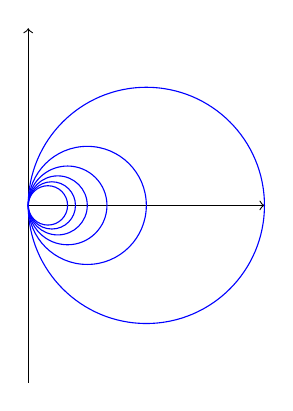
\begin{tikzpicture}[scale=1.5]
        %\draw[help lines] (0,-3) grid (3,3);

        \draw[->] (0,-1.5) -- (0,1.5);
        \draw[->] (0,0) -- (2,0); 
        \foreach \n in {1,...,6}
            \draw[blue] (1/\n,0) circle (1/\n);
    \end{tikzpicture}
    \caption{Two examples of sets which are rectifiable, but not manifolds.}
\end{figure}

Having shown that $\scrH^k \restrict T_p M$ is a tangent measure to $\scrH^k \restrict M$ for any $k$-dimensional Lipschitz submanifold $M \subseteq \bbR^d$ and $\scrH^k$-a.e. $p \in M$, we now ask when is the opposite true? Namely, can we judge that a set is a submanifold by showing it has approximate tangent spaces a.e., where an \textit{approximate tangent space} to a set $S \subseteq \bbR^d$ at $p \in S$ is a $k$-dimensional vector space $V \subseteq \bbR^d$ such that $\scrH^k \restrict V \in \Tan(\scrH^k \restrict S,p)$. Immediately, we see this is not true at all, as illustrated by figure \ref{fig:rectifiable}. First, the union of the $x$-axis and the parabola $y = x^2$ in $\bbR^2$ has an approximate tangent space at every point, but it fails to be a manifold near the origin.

More absurdly, take $H$ to be the union of circles centered at $(\frac{1}{n},0)$ with radius $\frac{1}{n}$ in $\bbR^2$ ($n \in \mathbb{N}$), the so-called \textit{Hawaiian earring}. The fundamental group $\pi_1(H)$ is famously complicated. In particular, it is uncountable, and therefore cannot be a topological manifold (see [Lee, Topological Manifolds, thm 7.21]). Despite this, it has approximate tangent spaces at a.e. point. Although since it exhibits some self-similarity at the origin, it is actually true that $\scrH^1 \restrict H$ is a tangent measure to itself at 0.

The thread linking our two counterexamples is that they are countable unions of submanifolds of $\bbR^d$, and this will turn out to be the correct generalization. We say a $\mathscr{H}^k$-measurable subset $E \subseteq \bbR^d$ is called $k$-\textit{rectifiable} if there exist Lipschitz maps $f_i \colon \bbR^k \to \bbR^d$, $i = 1,\dots,\infty$, such that 
\begin{equation}
    \mathscr{H}^k\left(E \setminus \bigcup_{i=1}^\infty f_i(\bbR^k)\right) = 0
\end{equation}
Rectifiable sets are in abundance. For a Borel set in $\bbR^d$ with locally finite perimeter, its measure-theoretic boundary turns out to be rectifiable. See \textbf{[Krantz \& Parks, Geometry of Domains in Space, §3.7]} for more information.

As a technical aside to state the next theorem, we need to quickly introduce Hausdorff densities. Fix a Radon measure $\mu \in \scrM(\bbR^d)$, a point $p \in \bbR^d$, and $s > 0$. Define the \textit{upper Hausdorff} $s$-\textit{density} of $\mu$ at $p$ to be
\begin{equation}
    \Theta^{s*}(\mu,p) := \limsup_{r \downarrow 0} \frac{\mu(B(p,r))}{r^s},
\end{equation}
and the \textit{lower Hausdorff} $s$-\textit{density} to be
\begin{equation}
    \Theta^s_*(\mu,p) := \liminf_{r \downarrow 0} \frac{\mu(B(p,r))}{r^s}.
\end{equation}
If both densities agree, we write $\Theta^s(\mu,p)$ for their common value, and call it the \textit{Hausdorff} $s$-\textit{density}.

The following theorem classifies the tangents of rectifiable sets.
\begin{theorem}\label{thm:rectifiableFlatSets}
    Fix $k \in \bbN$, and let $E \subseteq \bbR^d$ be $\mathscr{H}^k$-measurable with finite $\mathscr{H}^k$-measure, and such that $\Theta_*^k(E,p) > 0$ for $\mathscr{H}^k$-a.e. $p \in E$. Then $E$ is $k$-rectifiable if and only if for $\mathscr{H}^k$-a.e. $p \in E$, there exists an $k$-dimensional vector subspace $V_p \subseteq \bbR^d$ such that $\Tan(\mathscr{H}^k \vert_E,p) = \set{ c \scrH^k \restrict V_p : c > 0 }$.
\end{theorem}
As with most other things in geometric measure theory, the proof of theorem \ref{thm:rectifiableFlatSets} is highly technical, involving study of the truncated ``light cone"-shaped set
\begin{equation}
    E \cap B(p,r) \cap \{ x \in \bbR^d : d(x-p,V) < s\left|x-p\right| \},
\end{equation}
where $r,s > 0$ and $V$ is a $k$-dimensional subspace of $\bbR^d$ (figure \ref{fig:cone}). See \textbf{[Mattila §§15-16]} for more details.

\begin{figure}
    \centering
    \begin{tikzpicture}
        %\draw[gray] (0,0) grid (10,5);

        \draw (1,1) -- (9,4);
        %\draw (8,5) -- ++(0.9,-2.4);
        \node[right] (V) at (9,4) {$V$};
        \draw[red] (2,0) -- (8,5);
        \draw[red] (5-3.9,2.4) -- (8+0.9,5-2.4);
        \node[above] (p) at (5,2.5) {$p$};
        \filldraw[red] (5,2.5) circle (0.05);
        \draw[blue] (5,2.5) circle (1.5);
    \end{tikzpicture}
    \caption{Truncated ``light cone'' around a point $p$}
    \label{fig:cone}
\end{figure}

More generally, a Radon measure $\mu \in \scrM(\bbR^d)$ is said to be $k$-\textit{rectifiable} if $\mu$ is absolutely continuous with respect to $\mathscr{H}^k$, and there exists a $k$-rectifiable Borel set $E \subseteq \bbR^d$ such that $\mu(\bbR^d \setminus E) = 0$. We can generalize theorem \ref{thm:rectifiableFlatSets} to measures in the following way:
\begin{theorem} \label{thm:rectifiableFlatMeasures}
    Fix $k \in \bbN$, and let $\mu \in \scrM(\bbR^d)$ be a Radon measure such that $0 < \Theta_*^k(\mu,p) \leq \Theta^{k*}(\mu,p) < \infty$ for $\mu$-a.e. $p \in \bbR^d$. Then $\mu$ is $k$-rectifiable if and only if for $\scrH^k$-a.e. $p \in \bbR^d$, there exists a $k$-dimensional vector subspace $V_p \subseteq \bbR^d$ such that $\Tan(\mu,p) = \set{ c \scrH^k \restrict V_p : c > 0 }$.
\end{theorem}
The additional condition on the upper Hausdorff density of $\mu$ is vital (at least for $d=1$), as we will see with the Preiss measure later.

A Radon measure $\mu \in \scrM(\bbR^d)$ on is called $k$-\textit{flat} if there exists a $k$-dimensional vector subspace $V \subseteq \bbR^d$ and $c \in (0,\infty)$ such that $\mu = c \mathscr{H}^k \restrict V$. In the case of the above Hausdorff density condition, Rectifiable measures are therefore the ``upper bound'' on measures with flat tangent measures.